\chapter{The ATLAS experiment at the Large Hadron Collider}\label{sec:atlas}
Exploring the nature of the Higgs particle requires collision energies on the \qty[]{}{TeV} scale. The \ac{lhc} is currently the most powerful particle accelerator making it the best available facility for studying the Higgs particle. The main reference for this section is \citep{aad2008atlas}.

\section{The Large Hadron Collider}
The \ac{lhc} is a circular proton proton collider with \qty[]{27}{km} circumference with a center-of-mass energy of $\sqrt{s}=\qty[]{13}{TeV}$. The two anticyclic proton beams are actually bunches containing $10^{11}$ protons that are brought to collisions at several points of the ring for the experiments performed at the \ac{lhc}. A measure of how tightly particles are packed in these bunches is the instantaneous luminosity and is characteristic to the collider
\begin{equation}
    L=\frac{1}{\sigma}\frac{\dint{N}}{\dint{t}}.
\end{equation}
It can be read as particle interactions per unit time and area. The area understood as the interaction cross-section of a particular process. The total recorded number of collision events can thus be calculated by summing the luminosity over time which gives with the integrated luminosity
\begin{equation}
    N=\sigma\cdot\int L dt=\sigma\cdot L_\mathrm{int}.
\end{equation}
For the full run 2 dataset used in this thesis the integrated luminosity for events good for physics analysis is \qty[]{140.1}{fb^{-1}} \citep{DAPR-2021-01}. When bunches are collided not only one but rather several proton-proton interactions are measured. Methods to disentangle several  interactions at a once improved over time so the mean number of interactions also called pile up increased during the data taking period as can be seen in figure \ref{fig:pileup}.
\begin{figure}
    \centering
    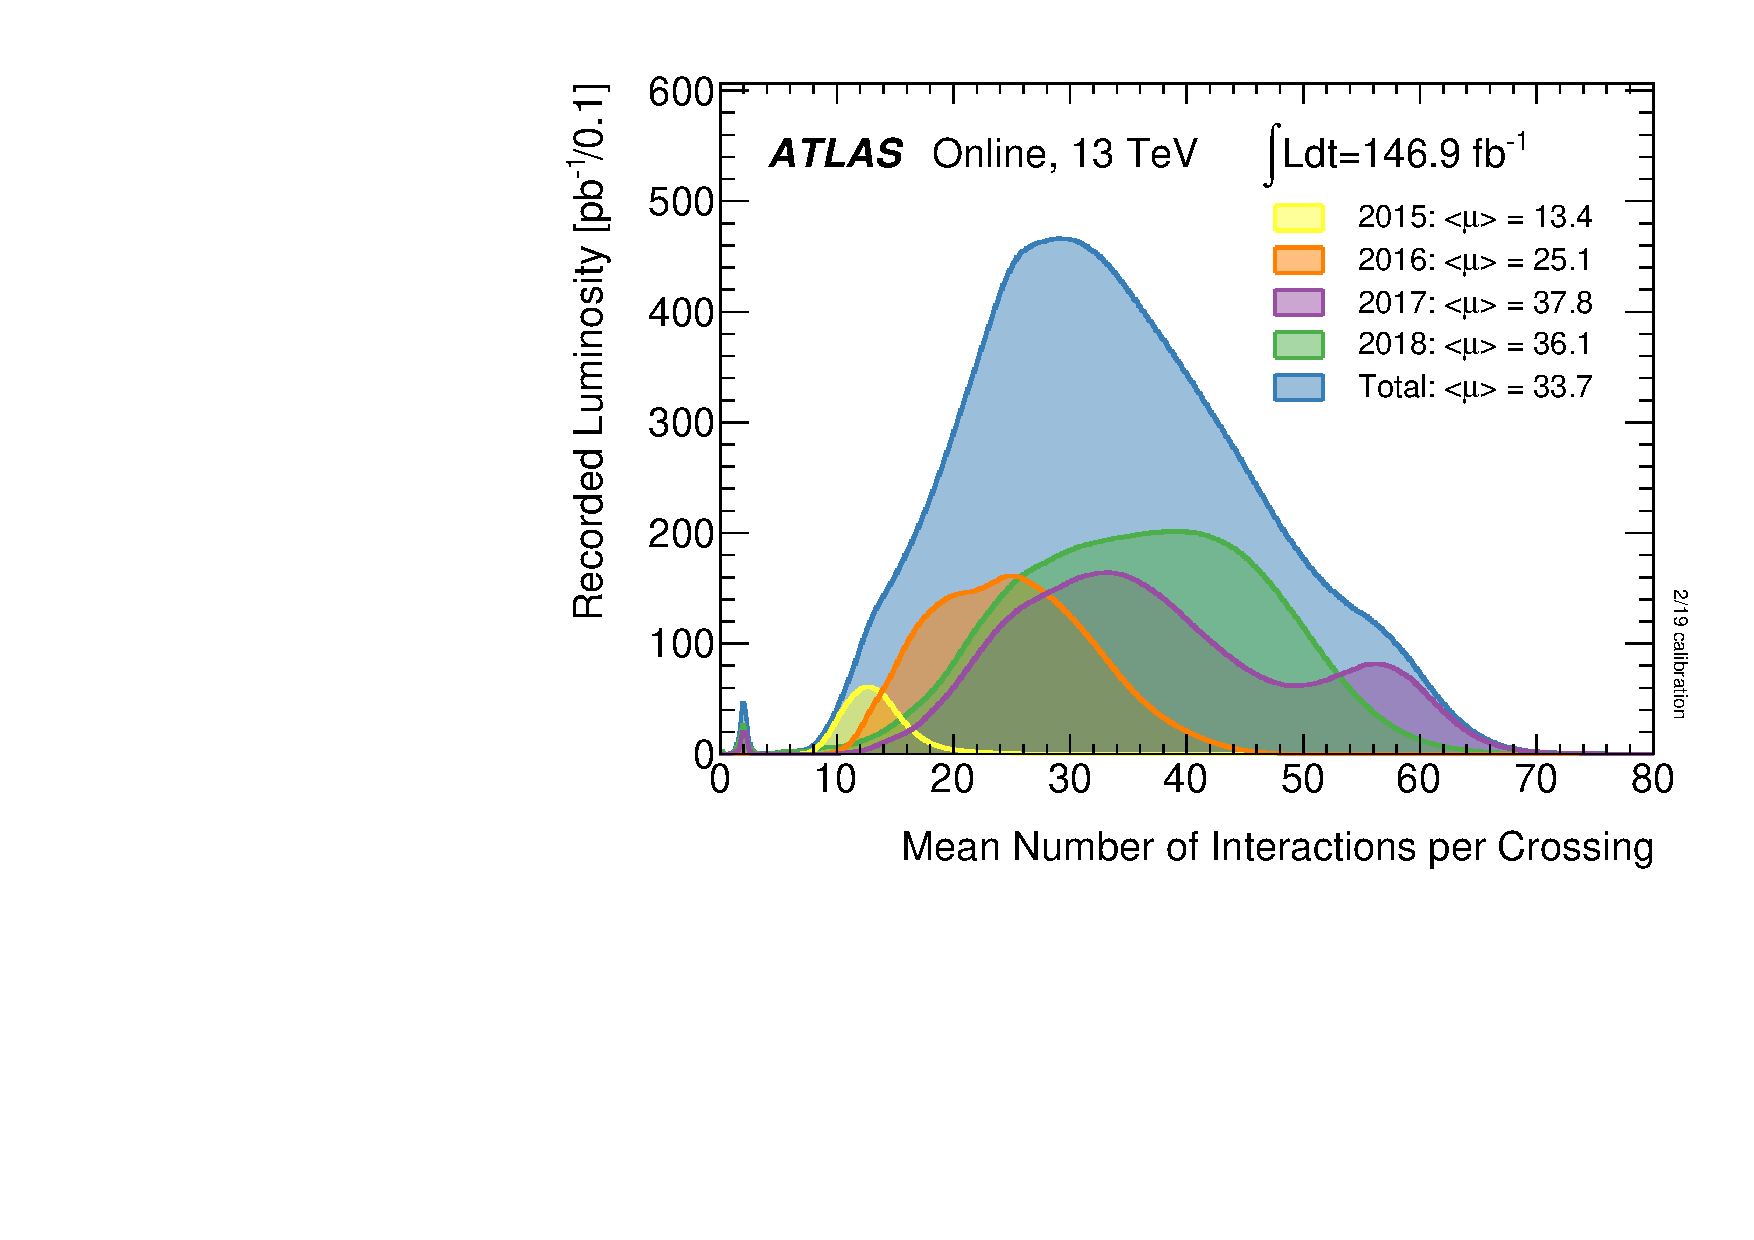
\includegraphics[width=0.5\textwidth]{mu_2015_2018}
    \caption[]{Pile up profiles for run 2 data taking periods \citep{pileup}.}
    \label{fig:pileup}
\end{figure}

\section{The ATLAS detector}
The \ac{atlas} (A Toroidal LHC Apparatus) experiment is a particle detector with an onion-like structure, as shown in figure \ref{fig:atlas_detector}.
\begin{figure}
    \centering
    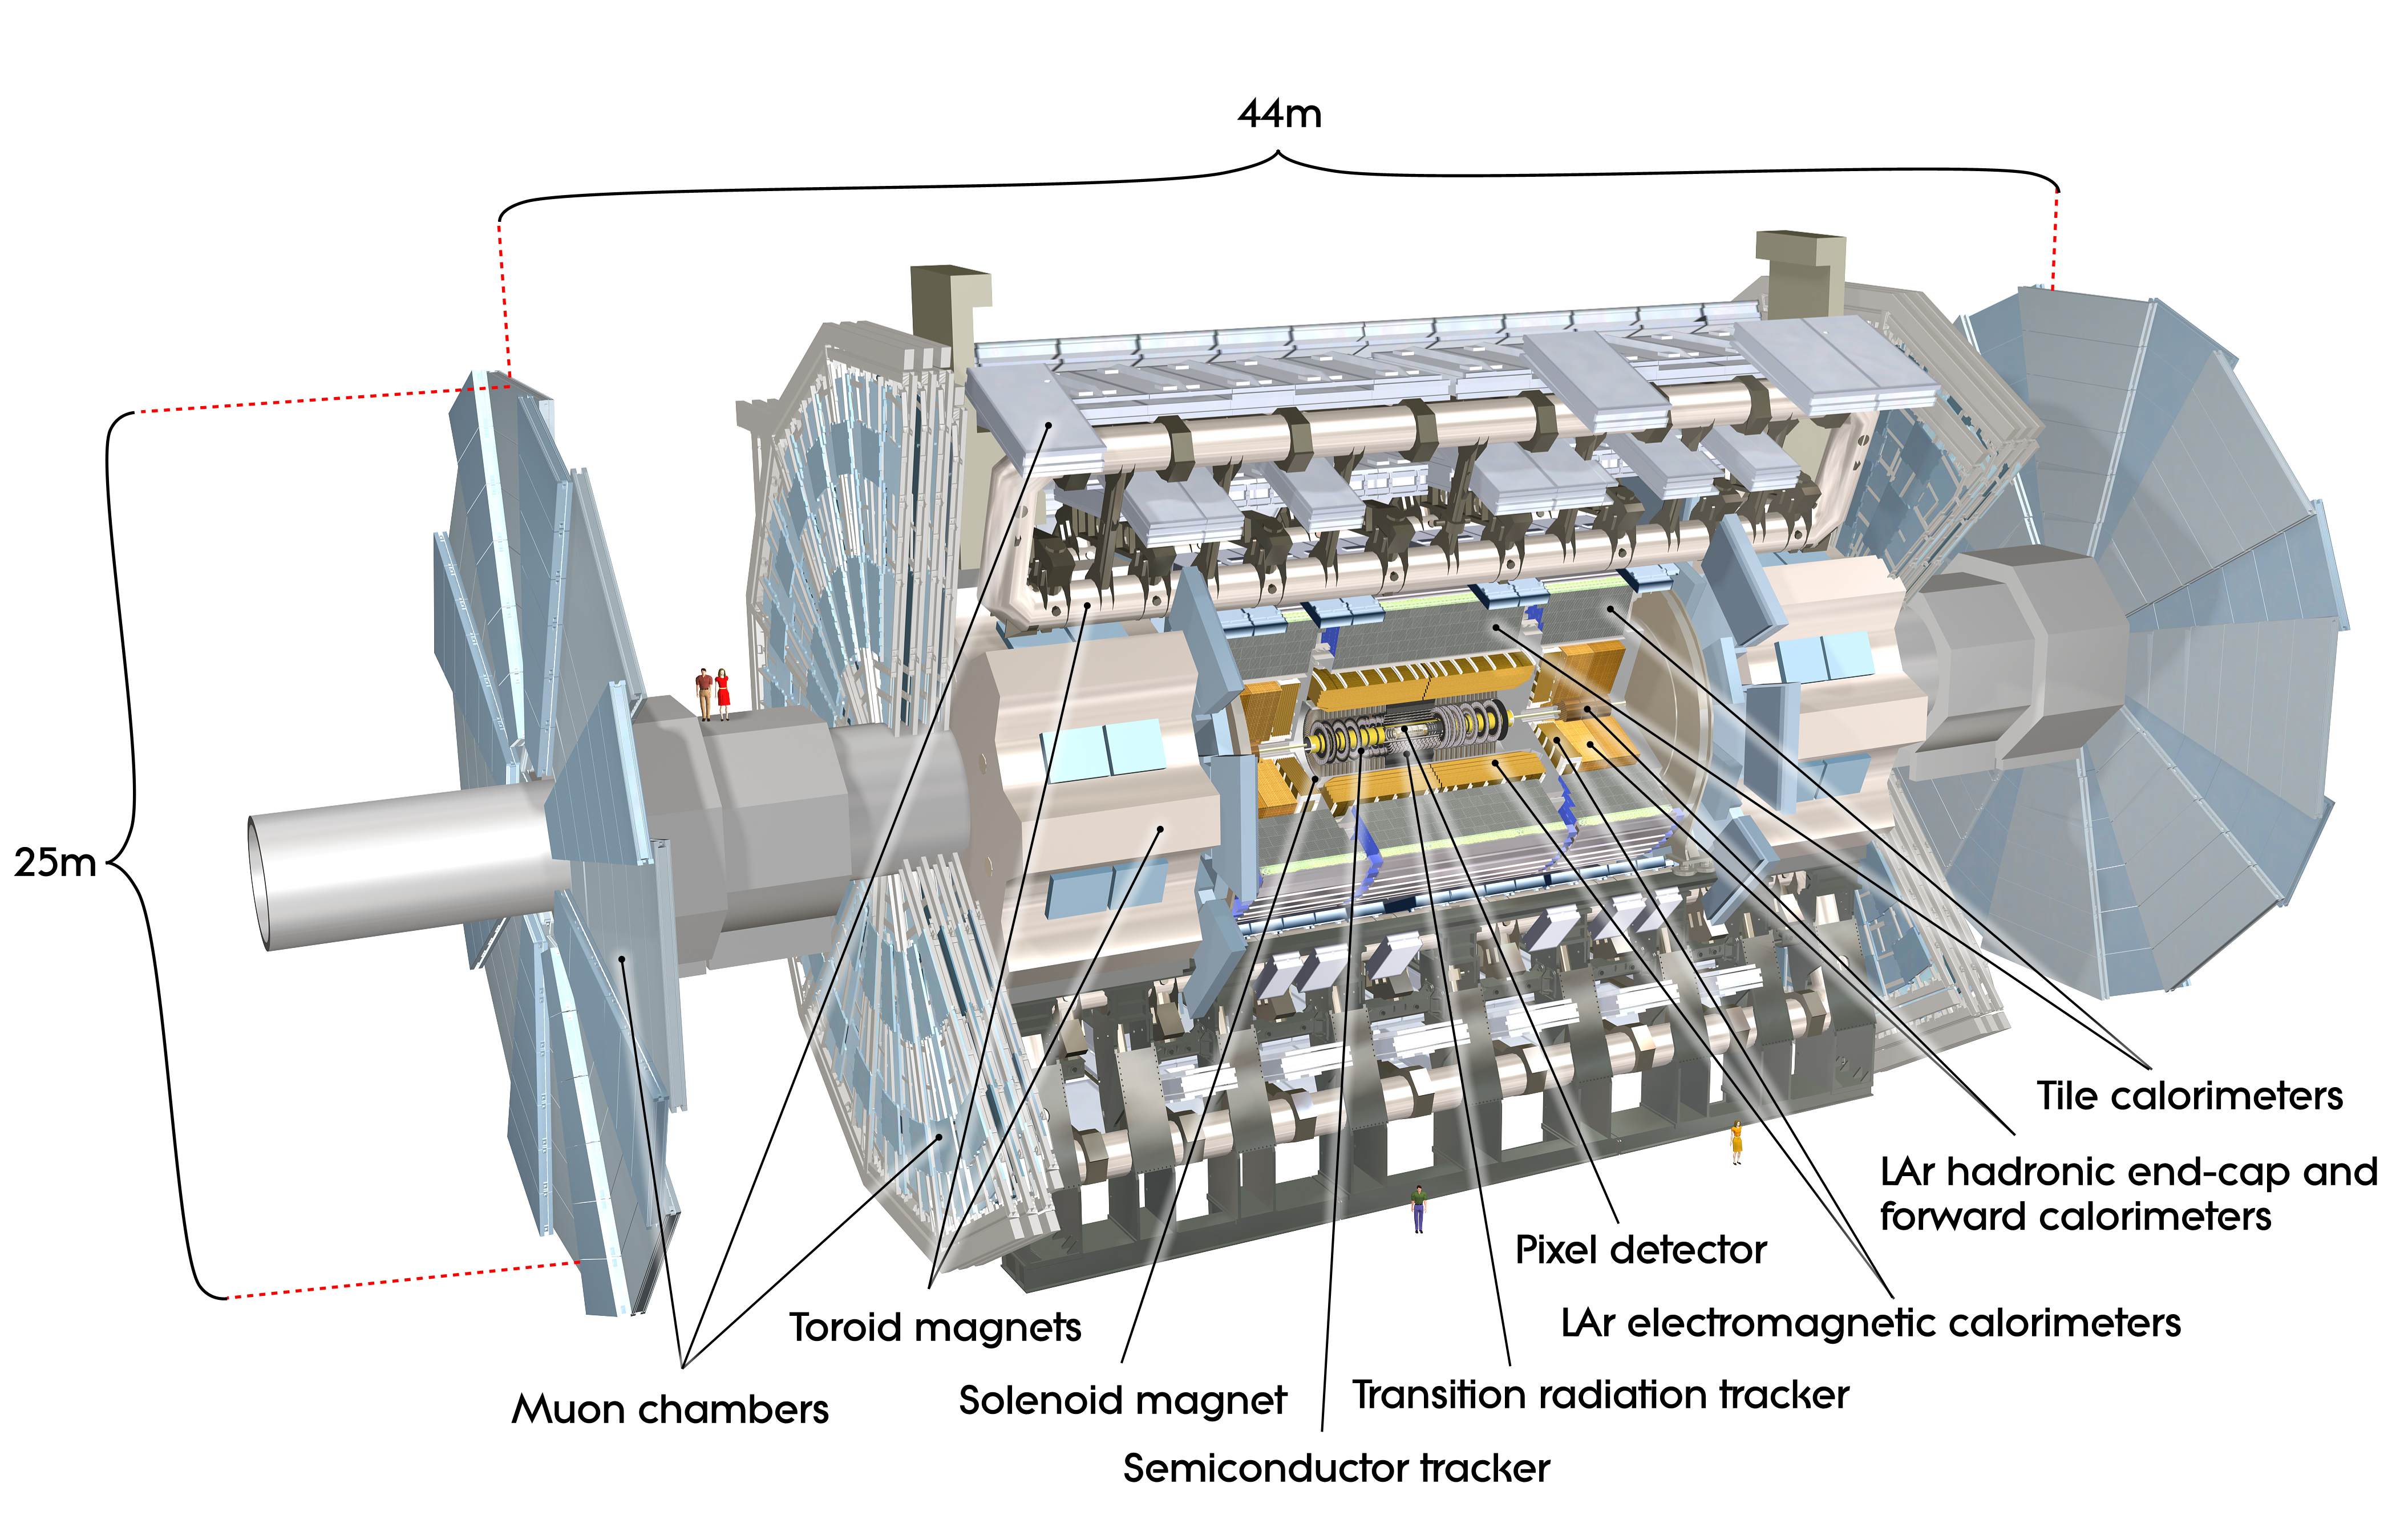
\includegraphics[width=1\textwidth]{atlas_detector}
    \caption[]{The \ac{atlas} experiment at the \ac{lhc} with its subdetectors. Adopted from \citep{Pequenao:1095924}.}
    \label{fig:atlas_detector}
\end{figure}
Its purpose is to measure the trajectory, momentum, and energy of particles originating from proton-proton collisions, depending on the particular kind of interaction of the collision products with matter. The various subdetectors are explained below from the inside out.

\subsection*{Coordinate System}
The coordinate system of \ac{atlas} is right-handed and originates at the interaction point at the center of the detector. The z-axis points along the beam line, the x-axis to the center of the lhc and the y-axis away from earth. Thus quantities transversal to the z-axis are Lorentz-invariant. Inside the detector cylindrical coordinates $r,\phi$ are used with $\phi$ the azimuthal angle about the z-axis and the polar angle $\Theta$ of a particle measured in form of the pseudorapidity $\eta=-\ln(\Theta/2)$. This quantity is defined as an approximation for the Lorentz invariant rapidity and holds for highly relativistic particles. With these a useful quantity to describe angular distances in the detector is
\begin{equation}
    \Delta R = \sqrt{(\Delta\phi)^2+(\Delta \eta)^2}.
    \label{eq:delta_R}
\end{equation}

\section{Inner detector}\label{sec:inner_detector}
The inner detector, shown schematically in figure \ref{fig:inner_tracker}, is designed to track charged particles and figure out their momentum and provide information on the particle type.
\begin{figure}
    \centering
    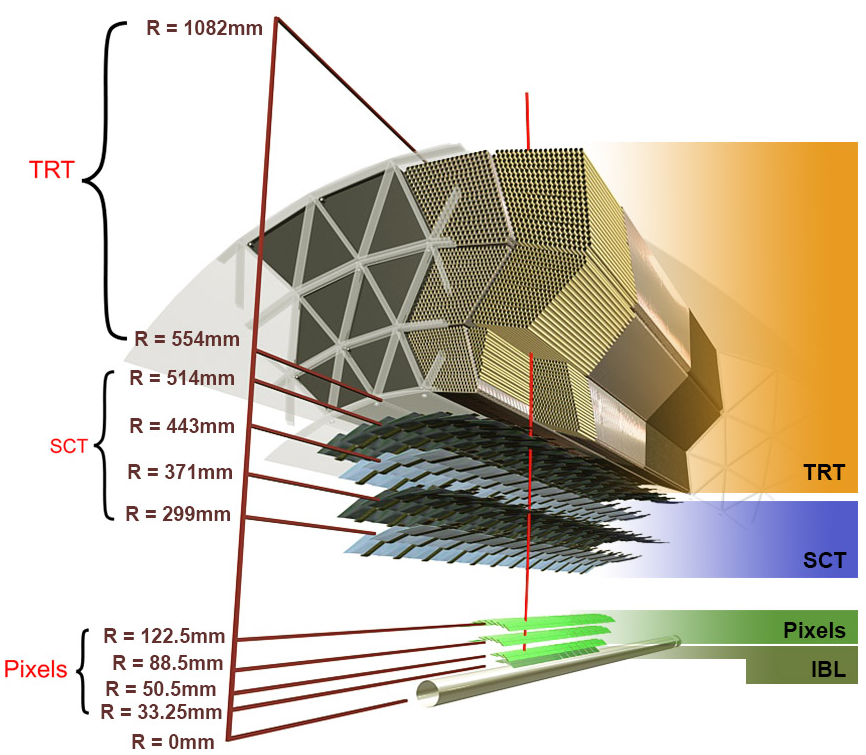
\includegraphics[width=0.65\textwidth]{inner_tracker}
    \caption[]{The inner detector schematically with the subdetectors described in the full text. Adopted from \citep{Potamianos:2016ptf}.}
    \label{fig:inner_tracker}
\end{figure}
It is surrounded by a solenoid magnet whose field lines point in the direction the beam so that charged particles are bent in the transverse plane of the detector due to the Lorentz force. The bending direction reveals the charge whereas the curvature depends on the momentum.

The \ac{ibl}, pixel detector, and \ac{sct} all consist of silicon detectors of various sizes. When passing through silicon, charged particles ionize electrons that travel in an electric field to an electrode and provide positional information. The \ac{ibl} plays a crucial role in b-tagging as will become clear in section \ref{sec:b_tagging}.

Aforementioned semiconductor trackers are surrounded by the \ac{trt} which apart from tracking also can identify particles. It consists of several layers of tubes perpendicular to the beamline, filled with a gas mixture, and a conducting wire in their center, which is under voltage and attracts negative charges. The tubes are surrounded in a material with different permittivity so that charged particles passing through the boundaries of the material emit transition radiation. The intensity of this radiation depends on the velocity, so that for particles of the same energy more photons are released for the lighter particle. Therefore for electrons for example can be distinguished from pions.

\section{Calorimeters}

When high-energy particles pass through dense matter the various particle interactions create secondary particles that result in a particle shower. Via this the energy of particles can be inferred and is done in \ac{atlas} with two sampling calorimeters. These consist of alternating layers of a high-density metal to absorb the energy and a material that can track the particles of the shower.

\subsection*{Electromagnetic Calorimeter}

In the electromagnetic calorimeter the main energy deposits are from electrons and photons. The stopping material consists of lead and steel and is alternated with a copper plate on which there is an electrode grid. Between the plates is liquid argon. When interacting with the dense metal e.g. by bremsstrahlung of an electron or by pair production induced by a photon, the created secondary particles ionize the argon atoms in between. The negatively charged ions are then pulled to the charged copper electrodes to determine the position. From the distance a particle has traveled through the electromagnetic calorimeter, one can infer the energy of the particle as it entered the calorimeter.

\subsection*{Hadronic Calorimeter}

Hadrons also deposit energy in the electromagnetic calorimeter but interact with nuclei as well. However as they are more energetic more stopping power is needed which is provided by the hadronic calorimeter that surrounds the electromagnetic calorimeter. The configuration is made of many layers of tiles positioned in planes perpendicular to the beamline. In these layers tiles of steel as stopping material alternate by a scintillating plastic which radiates light if charged particles pass through. The light is collected at the edges by wavelength-shifting optical fibres  which reduce the energy of the photons and then read out by photomultiplier tubes.

\section{Muon Spectrometer}

The muon spectrometer encircles all other detectors to capture muons which barely loose energy passing through the other detectors. Its basic units are resistive plate chambers in three layers around the calorimeters. These are basically large charged capacitors filled with gas. When charged particles pass through they ionize the gas and the resulting avalanche of ions drawn to the electrodes is measured to determine the position and time of flight through the plates.  In addition, they are also used in a design where the electrodes consist of a tube filled with gas and a wire inside similar to the \ac{trt}. The entire spectrometer is placed in a toroidal magnetic field so that the field lines are in phi direction in order to also measure the momentum due to the curvature of the muons.

The figure \ref{fig:particles_in_detector} shows where which type of particles are stopped in the different detectors.
\begin{figure}
    \centering
    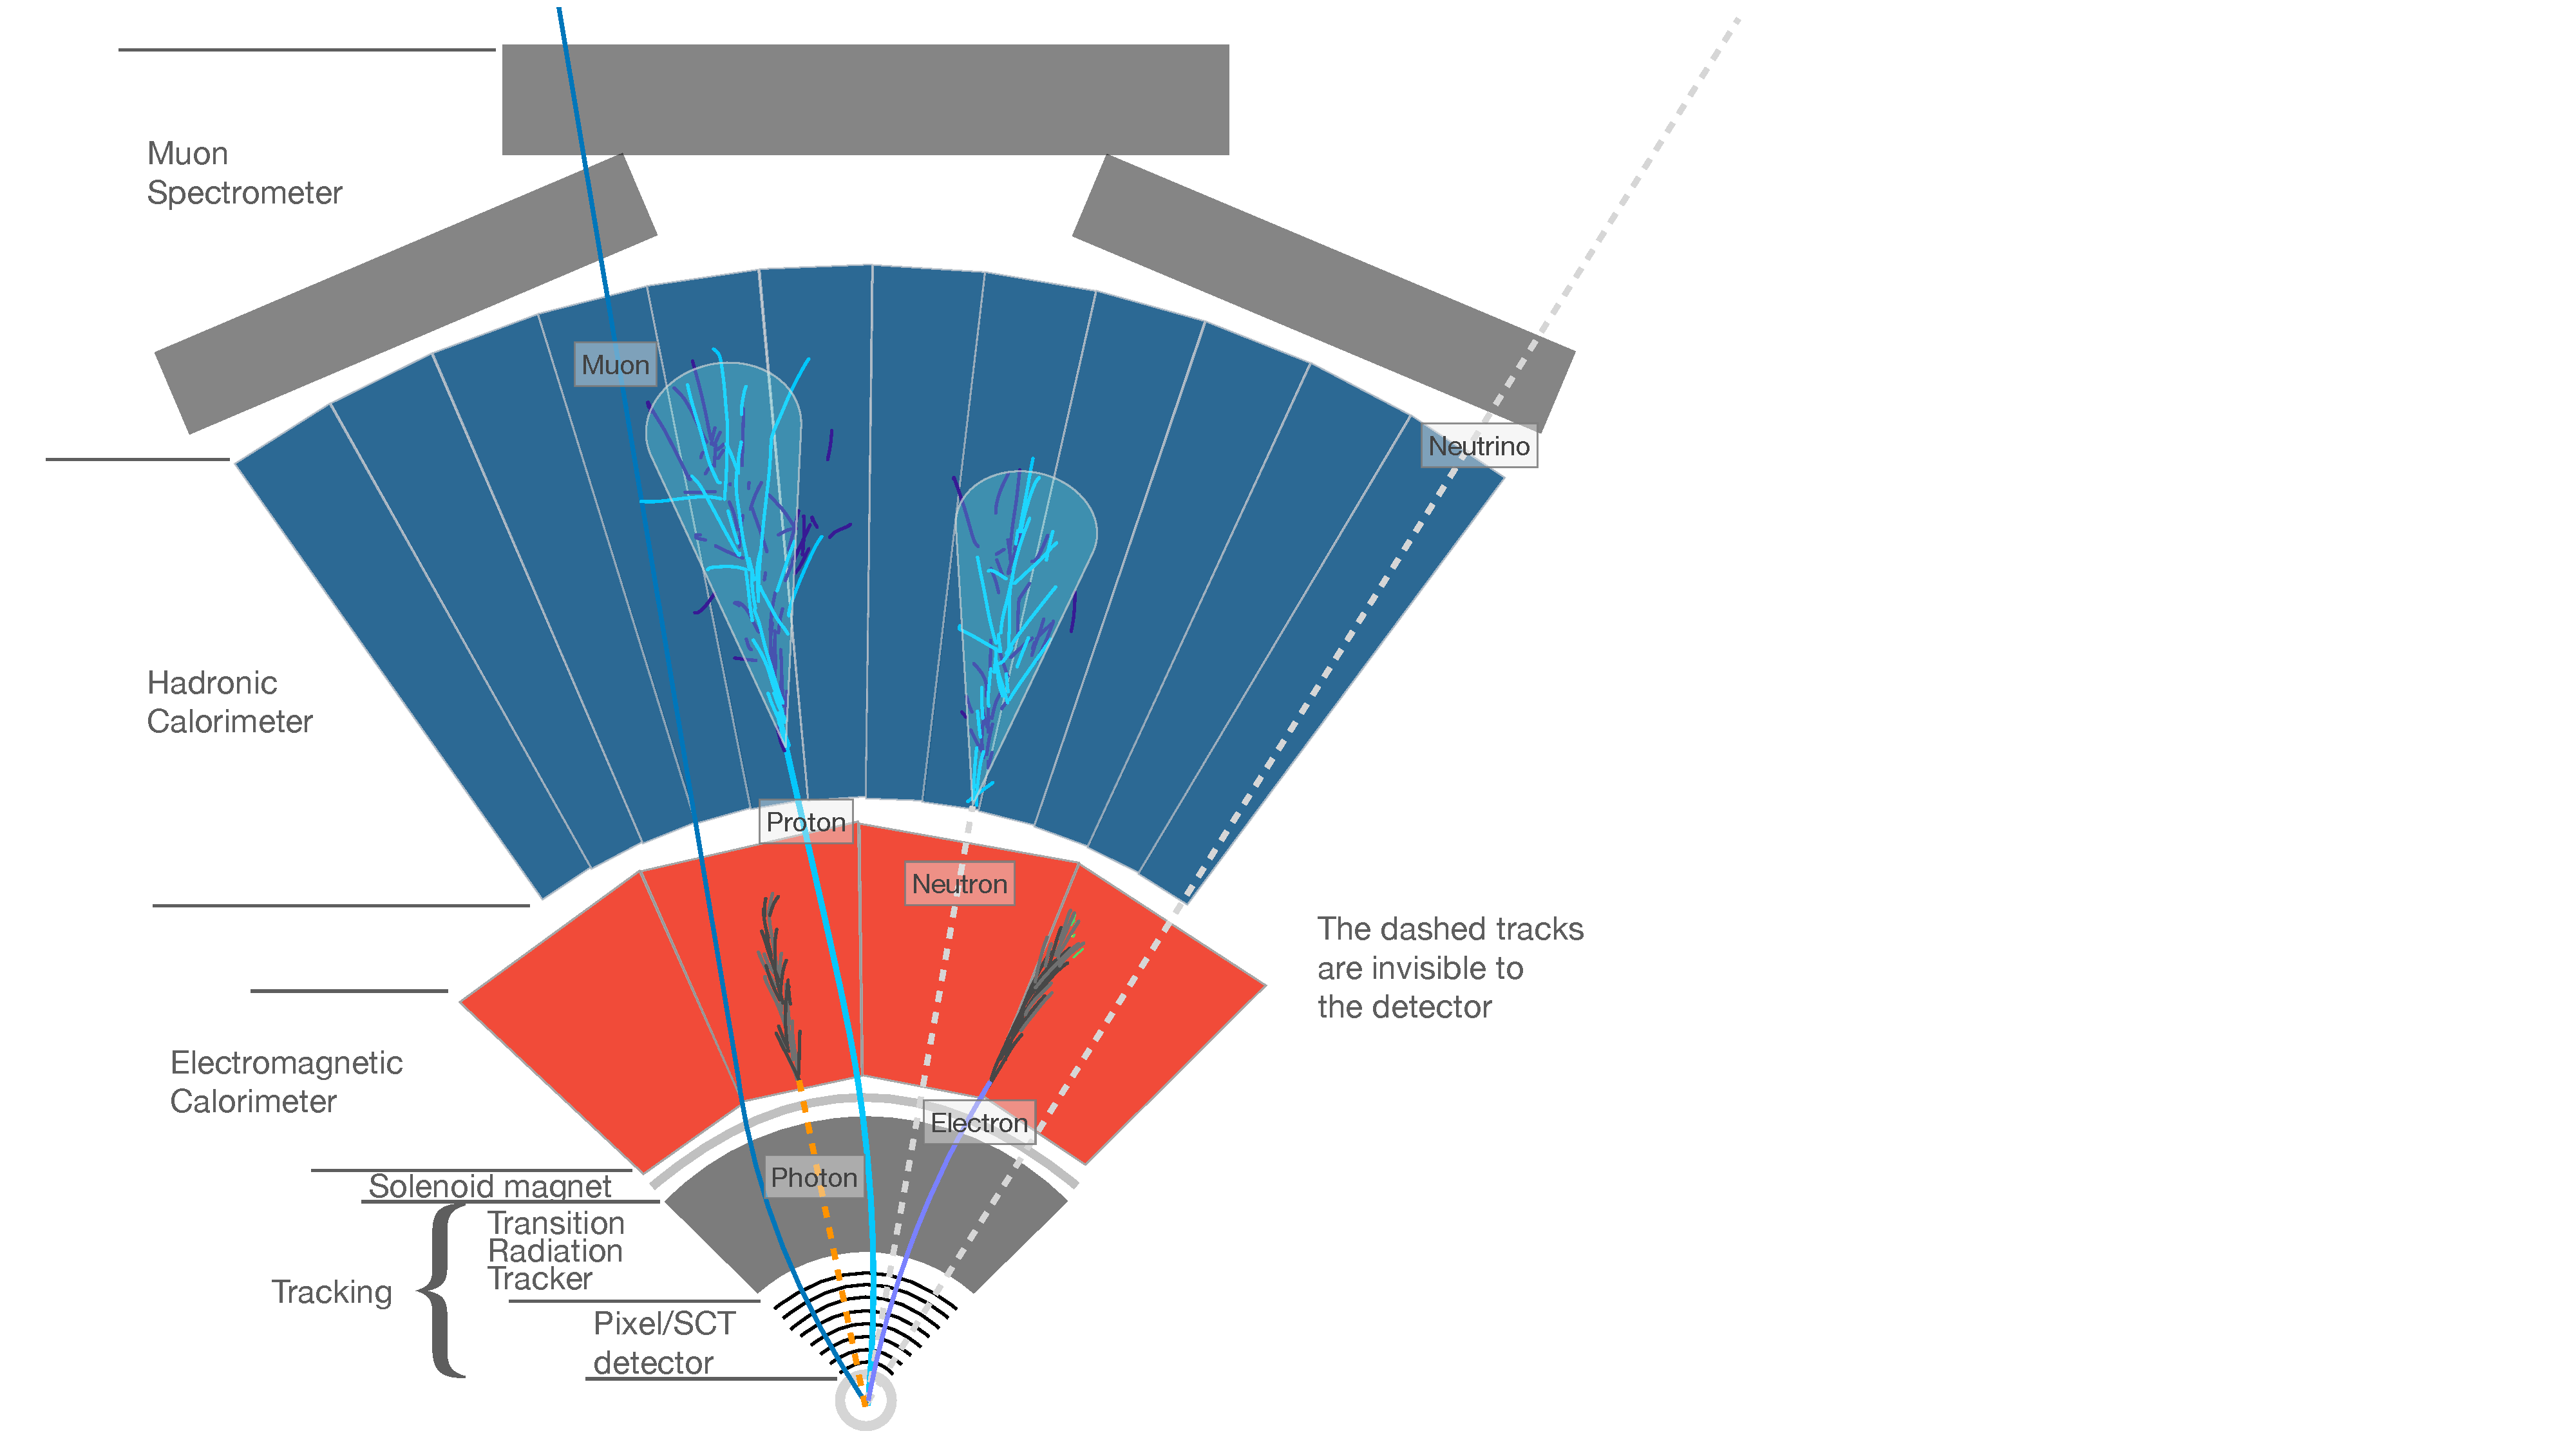
\includegraphics[width=1\textwidth]{particle-shower}
    \caption[]{Paths and energy deposits of particle types in the subdetectors. Adopted from \citep{Guth:2765038}.}
    \label{fig:particles_in_detector}
\end{figure}

\section{Data Acquisition}
Bunches of protons in the \ac{lhc} are brought to collision in \ac{atlas} with a rate of \qty[]{40}{MHz}. It is technically impossible at the moment to record all collisions as this would correspond to a data rate of \qty[]{40}{TB\per s}. Therefore events that are useful for physics analysis need to be preselected which is called triggering and is performed in two steps. The first step is the \ac{l1} trigger and is hardware based and reduces the event rate to \qty[]{100}{kHZ}. This is done by selecting events with large transverse momentum deposits in the detector and also for events with missing transverse momentum. Afterwards the regions in the detector where this is the case are passed to a software \ac{hlt}. This then uses the full detector information in these regions to reduce the rate further down to \qty[]{1}{kHz}.
